\documentclass[a4paper]{article}
\usepackage{labreport}

\begin{document}

\section{Objective}
The objective of the lab is to utilize the Thevenin and Norton methods to calculate the current and voltage across any one of several resistors in a circuit and verify the calculated values by measuring the values in the circuits \cite{UNCC-ECE-Dept:2023}.
\section{Equipment Used}

\begin{itemize}
    \item Digital Multimeter
    \item DC Power Supply
    \item Resistors: $1.2k\Omega$, $3.3k\Omega$, $10k\Omega$
\end{itemize}

\section{Experiment Setup}
To find the calculated values complete this procedure
\begin{enumerate}
    \item Remove the load resistor based off the model in Figure 9-1.
    \begin{center}
        \begin{figure}[H]\label{fig9-3}
            \begin{center}
                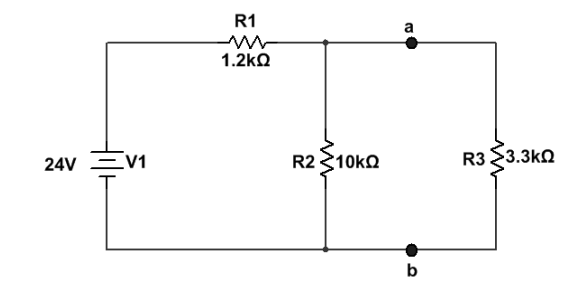
\includegraphics[width = 8cm]{Fig9-3}\\
                \small\textbf{Figure 9-1: Circuit for Thevenin and Norton Analysis \cite{UNCC-ECE-Dept:2023}}
            \end{center}
        \end{figure}
    \end{center}
    \item Calculate the thevenin voltage by calculating the voltage across the resistor in parallel with the open terminals.
    \item Calculate the resistance by removing current and voltage sources and replacing them with open and short circuits then calculate the equivalent resistance.
    \item For Norton equivalent repeat step 3 to calculate the resistance.
    \item To calculate norton current short the terminals and and calculate the current in the circuit.
\end{enumerate} 
\vspace{.5cm}
Lab Procedure for measurements
    \begin{enumerate}
        \item Construct the circuit in Figure 9-1 and measure the current in R3.
        \item Remove R3 and measure the voltage across the terminals.
        \item Reconnect R3 then measure the voltage and current in R3.
        \item Build the circuit in figure 9-4 and measure the Norton Current
        \begin{center}
            \begin{figure}[H]\label{fig9-4}
                \begin{center}
                    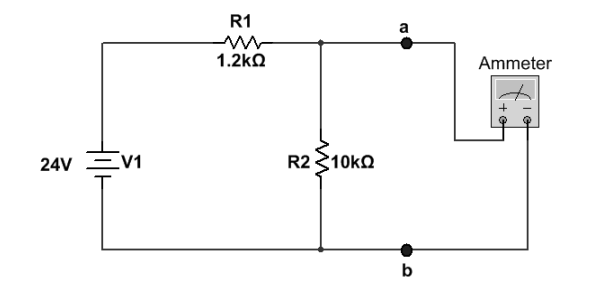
\includegraphics[width = 8cm]{Fig9-4}\\
                    \small\textbf{Figure 9-2: Circuit for Norton Analysis with R3 replaced by an Ammeter \cite{UNCC-ECE-Dept:2023}}\\
                \end{center}
            \end{figure}
        \end{center}
        \item Change the Ammeter with Ohmmeter and short the voltage source to measure the Norton resistance.
    \end{enumerate}
     


\section{Results}

\begin{center}
    \small\textbf{Table 9-1: Calculated Voltage and Current for Resistor R3 \cite{UNCC-ECE-Dept:2023}}
    \begin{tabular}{|p{3 cm}|p{3cm}|p{3 cm}|}
        \hline
         & Thevenin Equivalent & Norton Equivalent\\
        \hline
        $I_{R3}$ & 4.9 mA & 4.9 mA  \\
        \hline
        $V_{R3}$ & 16.17 V & 16.17 V  \\
        \hline
        
    \end{tabular}
\end{center}

\begin{center}
    \small\textbf{Table 9-2: Measured Thevenin and Norton Equivalents \cite{UNCC-ECE-Dept:2023}}
    \begin{tabular}{|p{3 cm}|p{3cm}|p{3 cm}|p{3 cm}|}      
        \hline
        \multicolumn{2}{|c|}{Thevenin Equivalent} & \multicolumn{2}{|c|}{Norton Equivalent}  \\
        \hline
        $v_{TH}$ & 21.43 V & $i_{N}$ & 18.3 mA \\
        \hline
        $R_{TH}$ & $1.056k\Omega$ & $R_{N}$ & $1.056k\Omega$ \\
        \hline
    \end{tabular}
\end{center}

\begin{center}
    \small\textbf{Table 9-3: Measured Voltage and Current for Resistor R3 \cite{UNCC-ECE-Dept:2023}}
    \begin{tabular}{|p{3 cm}|p{3 cm}|p{3 cm}|p{3 cm}|}
        \hline
        & Figure 9-3 & Thevenin Equivalent & Norton Equivalent \\
        \hline
        $I_{R3}$ & 4.961 mA & 4.961 mA & 4.596 mA \\
        \hline
        $V_{R3}$ & 16.19 V & 16.18 V & 15 V\\
        \hline
    \end{tabular}
\end{center}



\section{Conclusion}

Thevenin and Norton equivalent circuits are way to reduce circuits to a simpler form that makes finding current though, voltage in, and resistance in a circuit. The Norton Current and Thevenin Voltage
will be the values across the load resistor. Norton Resistance equals Thevenin Resistance and the Thevenin Voltage is equal to the Thevenin Resistance times the Norton Current.  

\bibliography{references}
\bibliographystyle{plain}



\end{document}